\section{Background and Related Work}
In this section, we briefly introduce the relevant work of scientific application from the aspect of task dependencies, then we introduce the workflow system that supports those using scenarios and explain the shortage of current workflow system, at last, we will introduce the pub-sub mechanism and it's using in the workflow system.

\subsection{Types of Scientific Application and Workflow System}
Considering the scientific application in \cite{makeflowexample}, the execution of tasks in workflow could be represented as DAG (Directed Acyclic Graph), every node represent the execution of the task and every edge represent the sequence of the execution between tasks. For workflow tool such as \cite{makeflowexample,wilde2011swift}, the abstraction of DAG should be fixed before the application running, the user should grasp the topology of the task dependency in advance and execute the workflow by submitting the description file, then workflow will schedule and execute the task according to this DAG blueprint. The intermediate file was used to control the execution of the typical dependency pattern\cite{bharathi2008characterization}.

There are other types applications without fixed and explicit task dependency pattern before the task running, the task may or may not be triggered during task running and it depends on the content of the data instead of the input/output data files in those cases. For example, in simulation-analyzing-visualization workflow, a large amount of simulation data will be generated in short time, some simulation will also running several days, there are some redundant data in the output of the data but only some of them are useful data. If we only want to visualize the data with the average value larger than the specific threshold, the picture will be plotted only when data satisfy our predefined condition. There are several strategies for workflow system to address this issue, one is post-processing which will load all the simulation data into the disk and then process the data in separate tasks. But this solution only useful for small-scale simulation, the increasing data, size and limited storage and bandwidth make high fidelity post-processing impractical\cite{ayachit2015paraview}. In situ workflow is the latest trend to solve this issue\cite{dreher2017situ}. There are several intermediate components to leverage the in-situ workflow\cite{docan2012dataspaces,ayachit2015paraview}  there are works exploring how to decompose original algorithm into in-situ method such as\cite{bennett2012combining} some works are exploring the properties of workflow at exascale\cite{dreher2017situ} but few works focusing on how workflow support different type of in-situ tasks involving flexible dependencies relationship. 

\subsection{Types of Dependencies between Workflow Tasks}
One critical distinction between the traditional workflow(without in-situ task) and the in-situ workflow is the construction of task dependencies. For traditional workflow such as \cite{albrecht2012makeflow}, the dependencies are determined by input and output files between tasks, for example, if the output file of task A is the input of task B there is a dependency between task A and task B namely task B needed to be started after taskA finish.  In the in-situ/in-transit/Hybrid workflow, the dependency will be described in much finer granularity and more flexible way.  For example, task B will start after one loop iteration of taskA finish, or taskB needed to be started when the output of taskA satisfy the specific condition. According to the Figure 1 in the introduction, this is a kind of hybrid pattern: the in-situ part will be used to detect if the interested happens and then the in-transit pattern will be triggered to analyze the data. Dedicated communication libraries needed to be used to send the message between different tasks to synchronize the execution of the task, namely to decide when the task is supposed to be started. No matter for the traditional task or in situ tasks, the task dependency pattern could be divided into three main types \cite{albrecht2012makeflow,bharathi2008characterization} which are shown in Figure 2. 
\begin{figure*} 
\centering
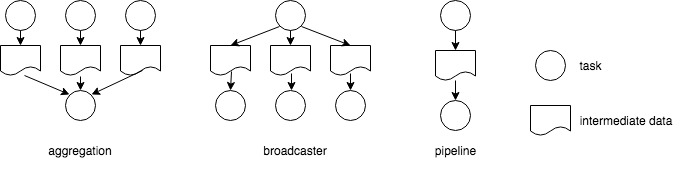
\includegraphics[width=.8\linewidth]{./figure/taskpattern.jpg}
\caption{typical workflow pattern}
 \label{fg:state}
\end{figure*} 

For traditional workflow, the intermediate data are files on the disk and the work queue\cite{albrecht2012makeflow} could be used to control the execution of tasks,  for in-situ workflow, one solution is to view the intermediate data as series of event messages which will be used to control the task execution sequence generated by in-situ tasks or infrastructure running the tasks.

\subsection{Pub-Sub paradigm and event-driven workflow pattern}

Once we assume event message as a special intermediate data used to synchronize the task execution, Pub-Sub paradigm \cite{eugster2003many} could satisfy the requirements to run fine granularity task dependency by messaging communication in the distributed way, There are also all kinds of implementation in research and industry using event message broker based on those pub-sub-notify architecture\cite{hivemq,jin2012scalable,redispubsub}, but there are few scientific workflow systems combining the task dependency and event driving programming together. Some works such as \cite{jin2012scalable} use this mechanism to leverage the in situ workflow, but they only support the specific underlying library and the types of task dependency pattern is also limited. A canonical pub-sub mechanism works in three steps , assume there are two component namely subscriber $S$ and publisher $P$ (1) $S$ will subscribe one or more interesting events into the pub-sub broker (2) $P$ will push events into the pub-sub broker (3)  pub-sub broker will notify $S$ if pushed event match the subscribed event. There exists a dependency between publisher and subscriber in this paradigm. If we use this programming model to compose workflow, the task could be a publisher or subscriber at in the workflow, there will be less restriction on task because any type of tasks could generate the event used to construct the dependency , the task can be in-situ part of the task or jobs running by sbatch system flexibly according to different using scenarios. By this task composing model,  This kind of event-driven workflow should support the task paradigm in Figure 3.
\begin{figure*} 
\centering
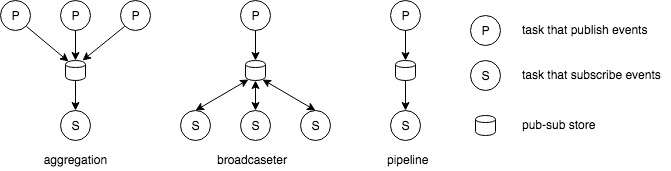
\includegraphics[width=.8\linewidth]{./figure/edtaskpattern.jpg}
\caption{typical event-driven workflow pattern}
 \label{fg:state}
\end{figure*} 
One advantage to use event message to express dependency is the flexibility for dependency granularity, the event message is an abstraction of the user-defined dependent data bock which could be the disk files or data instance in memory. 
There are following scenarios to use event programming to leverage scientific workflow:

(1)Event messages could also represent the properties of data and runtime, for example, an event could represent data in a specific domain is larger than a threshold

(2)The status of underlying infrastructure, the start, stop of runtime system(batch runtime system or container runtime system)

(3)In-situ, in-transit and post-processing tasks can be composed together in a workflow by event message abstraction

The broadcaster and pipeline pattern are supported by pub-sub-notify mechanism naively but there is no support for aggregation pattern. For typical pub-sub mechanism, is subscriber subscribe multiple events such as eventA, eventB eventC, and publishing of those three events will notify the subscriber and trigger execution of task, however, in workflow aggregation scenario, the specific subscribed runtime is supposed to be triggered when all eventA , eventB and eventC are published and satisfied. We will discuss the details of pub-sub event store and relevant runtime client to support all of those patterns in implementation part. 
